\chapter{Simple Machines}

As mentioned earlier, physicists define work as the force applied times the 
distance over which it is applied. For example, if you push your car 100 meters 
with a force of 17 newtons, you have done 1700 joules of work.

Humans have long needed to move heavy objects, so many centuries ago, we 
developed simple machines to reduce the amount of force necessary to perform 
such tasks. These include:

\begin{itemize}
    \item Levers
    \item Pulleys
    \item Inclined planes (ramps)
    \item Screws
    \item Gears
    \item Hydraulics
    \item Wedges
\end{itemize}

\includegraphics[width=\textwidth]{simplemachines.png}

While these machines can reduce the force needed, they do not change the total 
amount of work that must be done. For instance, if the force is reduced by a 
factor of three, the distance over which the force must be applied \textit{increases} by 
the same factor.

\section{Mechanical Advantage}

Mechanical advantage is the ratio between the force output 
by the machine and the force the user puts into the machine:
$$ MA = \frac{F_{out}}{F_{in}} = \frac{Load}{Effort}$$

Since the input force is \textit{applied} to the simple machine, sometimes the 
input force is called an applied force and abbreviated as $F_a$. For example, 
you only need to apply a relatively little force to your car's brakes in order 
for the hydraulic braking system to apply enough force to your tires to stop 
them spinning (we'll examine this further below). 

\subsection{What does it mean to work hard?}
Humans use simple machines to ``make work easier", but what does this mean in a 
physics sense? Does using a machine actually decrease the amount of work the 
user has to do? When we say a task is easier, we usually mean \textit{we have to 
apply less force}. You might say that it is ``less work" to push something up a 
shallow incline than up a steep incline. But does the person pushing \textit{
actually do less work} (in a physics sense), or does that work simply require 
a smaller force? We'll answer this question by examining the physics of incline 
planes below, and the results will be true for all simple machines. 

Ideally we want a higher Mechanical Advantage, which means we are putting in less input force for a greater output force.
\section{Inclined Planes}

Inclined planes, or ramps, allow you to roll or slide objects to a higher 
level. Steeper ramps require less mechanical advantage. For instance, it is much 
easier to roll a ball up a wheelchair ramp than a skateboard ramp.

\includegraphics[width=\textwidth]{rampcomparison.png}

Assuming the incline has a constant steepness, the mechanical advantage is 
equal to the ratio of the length of the inclined plane to the height it rises. 
%note to self: show why this is true or have students derive eqn in exercise -Max

If friction is neglected, the force required to push a weight up the inclined 
plane is given by:
\begin{equation}
    F_A = \frac{V}{L} F_g 
    \label{eq:forceIncPlane}
\end{equation}
\
% also explain why v and l is the inverse of mechanical advantage
% state that L is the hypotenuse formed by the tringle
where \( F_A \) is the applied force, \( L \) is the length of the inclined plane, \( V \) is the vertical rise, and \( F_g \) is the gravitational force acting on the mass.

\begin{center}
	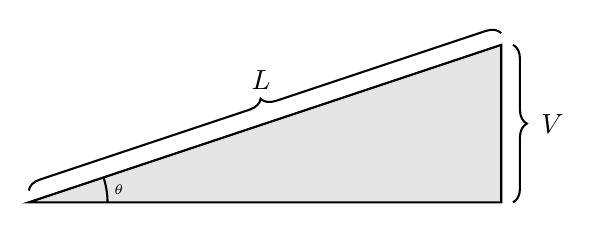
\begin{tikzpicture}
	   \draw[thick, black, fill=gray!20] (0,0) -- (6, 0) -- (6, 2) -- cycle;
          \draw[black] (1, 0) arc (0:18:1) 
          	node[font=\tiny, right, yshift = -0.15cm] {$\theta$};
          \draw[decorate, decoration = {brace, amplitude=5pt}] 
          	(0, 0.15) -- (6, 2.15);
          \node[] at (2.95, 1.55) {$L$};
          \draw[decorate, decoration = {brace, amplitude=5pt, mirror}] 
          	(6.15, 0) -- (6.15, 2);
          \node[] at (6.65, 1) {$V$};
	\end{tikzpicture}
\end{center}

(We will discuss sine function later, but in case you're familiar with it, note that:

\begin{equation}
    \frac{V}{L} = \sin{\theta}
    \label{eq:incPlaneSinDeriv}
\end{equation}


where \( \theta \) is the angle between the inclined plane and the horizontal surface.)

Let's compare the force needed and work done when pushing a load up a ramp 
versus just lifting it vertically. Consider a family on moving day: there's a 
hand trolley loaded with 200 N (about 45 pounds) of boxes. If the bed of the 
moving truck is 1.5 m high, how much work would it take to lift the boxes 
straight up into the truck? What about with a ramp? 

First, let's look at how much force and work is needed if you were to lift the 
entire 200 N load straight up into the air. You'd need to apply 200 N of force 
upwards for a distance of 1.5 m:
$$W = F \cdot d = \left( 200 \text{ N} \right) \left( 1.5 \text{ m} \right) = 300 \text{ J}$$

So, without a ramp, you would have to apply 200 N and do 300 J of work. Suppose 
your moving truck comes with a ramp that has an incline of 15 degrees:

\begin{center}
	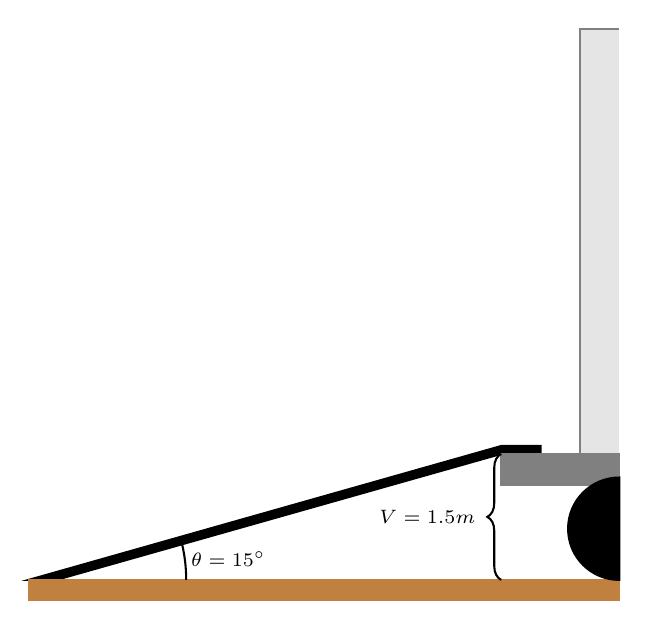
\begin{tikzpicture}
            \draw[black, fill=black] (0,0) -- (6, 1.7) -- (6.5, 1.7) -- 
            	(6.5, 1.6) -- (6, 1.6) -- (0.35, 0) -- cycle; 
	    	\draw[gray, fill=gray] (6, 1.2) rectangle (7.5, 1.6);
            \draw[brown, fill=brown] (0,-0.25) rectangle (7.5, 0);
            \draw[black, fill=black] (7.5, 1.3) arc (90:270:0.65) -- cycle;
            \draw[gray, fill=gray!20] (7.5, 1.6) -- (7, 1.6) -- (7, 7) -- (7.5, 7);
            \draw[black] (2, 0) arc (0:15:2) 
            	node[right, yshift = -0.25cm, font = \scriptsize] 
            	{
            	$\theta = 15^{\circ}$
            	};
            \draw[decorate, decoration = {brace, amplitude=5pt, mirror}] 
            (6, 1.6) -- (6, 0) 
            node[left, yshift = 0.8cm, xshift = -0.2cm, font = \scriptsize] 
            {
            $V=1.5\text{ m}$
            };
	\end{tikzpicture}
\end{center}

Since $\sin{ \left( \theta \right) } = V/L$, we know that $L = V / \sin{ \left( 
\theta \right) }$. You can use a calculator or search engine to find that the 
sine of $15^{\circ} \approx 0.26$. Therefore, the length of the ramp is 
approximately 5.8 meters. How much force does it take to move the load of boxes 
up the ramp? Intuitively, we know it is less force. We can use a 
\newterm{free body diagram} to determine the minimum force needed to push the 
box up the ramp. \index{free body diagram}(A free body diagram is a simplified 
model showing all the forces acting on an object. You'll learn to create and 
use your own free body diagrams in a later chapter. For now, just follow along.)

Before you push it, there are two forces acting on the loaded hand trolley: its 
weight ($F_g$) and the normal force between the trolley and the ramp ($F_N$):

\begin{center}
	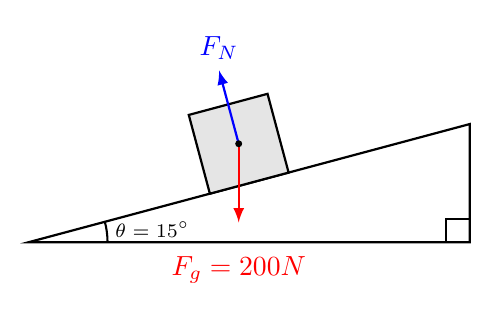
\begin{tikzpicture}
            \draw[thick, black] (0,0) -- (5.6, 0) -- (5.6, 1.5) -- cycle;
            \draw[] (5.3, 0) -- (5.3, 0.3) -- (5.6, 0.3);
            \draw[] (1, 0) arc (0:15:1) node[right, font = \scriptsize, yshift = -0.1cm] 
            	{$\theta = 15^{\circ}$};
            \draw[thick, black, fill=gray!20] (2.3, 0.616) -- (3.3, 0.884) -- 
            	(3.032, 1.884) -- (2.032, 1.616) -- cycle;
            \draw[-latex, thick, blue] (2.666, 1.25) -- (2.416, 2.183) 
            	node[above] {$F_N$};
            \draw[-latex, thick, red] (2.666, 1.25) -- (2.666, 0.25) 
            	node[below, yshift = -0.3cm] {$F_g = 200\text{ N}$};
            \draw[black, fill=black] (2.666, 1.25) circle (0.03cm);
	\end{tikzpicture}
\end{center}

Notice that the normal force is perpendicular to the ramp! We want to know how 
much force it takes to push the load up the ramp, so we will ``split" the 
weight force vector into two parts: one part parallel to the ramp ($F_{g,\vert 
\vert}$) and one part perpendicular ($F_{g, \perp}$):

\begin{center}
	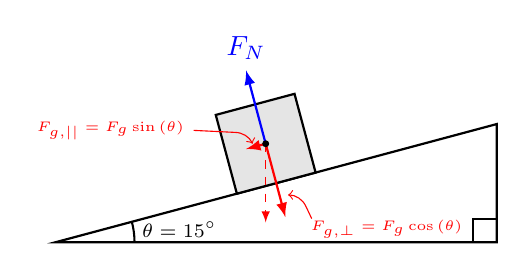
\begin{tikzpicture}
            \draw[thick, black] (0,0) -- (5.6, 0) -- (5.6, 1.5) -- cycle;
            \draw[] (5.3, 0) -- (5.3, 0.3) -- (5.6, 0.3);
            \draw[] (1, 0) arc (0:15:1) 
            	node[right, font = \scriptsize, yshift = -0.1cm] 
            	{$\theta = 15^{\circ}$};
            \draw[thick, black, fill=gray!20] (2.3, 0.616) -- (3.3, 0.884) -- 
            	(3.032, 1.884) -- (2.032, 1.616) -- cycle;
            \draw[-latex, thick, blue] (2.666, 1.25) -- (2.416, 2.183) 
            	node[above] {$F_N$};
            \draw[-latex, thin, red, dashed] (2.666, 1.25) -- (2.666, 0.25);
            \draw[-latex, thick, red] (2.666, 1.25) -- (2.916, 0.317);
            \draw[-latex, thick, red] (2.666, 1.25) -- (2.416, 1.183);
            \draw[black, fill=black] (2.666, 1.25) circle (0.03cm);
            \draw[red, <-, thin] (2.95, 0.6) arc (90:25:0.25) -- (3.25, 0.3) 
            	node[below, font = \tiny, xshift = 0.95cm, yshift = 0.1cm] 
            	{$F_{g,\perp} = F_g \cos{\left( \theta \right)}$};
            \draw[red, <-, thin] (2.5, 1.25) arc (25:90:0.25) -- (1.75, 1.42) 
            	node[left, font = \tiny] 
            	{$F_{g,\vert \vert} = F_g \sin{ \left( \theta \right)}$};
	\end{tikzpicture}
\end{center}

We did this by treating the weight vector as the hypotenuse of a right triangle 
with legs perpendicular and parallel to the ramp. You'll learn how to do this 
and why it works in the chapter on vectors. For now, just trust that the part 
of the hand trolley's weight that is perpendicular to the ramp is $F_g \cos{ 
\left( \theta \right) }$ and the part that is parallel to the ramp is $F_g 
\sin{ \left( \theta \right) }$.

What force do you need to overcome to push the hand trolley up the ramp? Just 
the part of the weight that is parallel to the ramp! You'll need to apply an 
equal force in the opposite direction (up the ramp) to move the hand trolley:

\begin{center}
	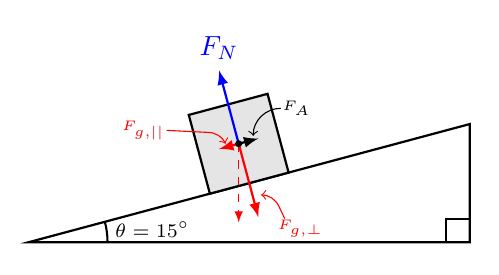
\begin{tikzpicture}
            \draw[thick, black] (0,0) -- (5.6, 0) -- (5.6, 1.5) -- cycle;
            \draw[] (5.3, 0) -- (5.3, 0.3) -- (5.6, 0.3);
            \draw[] (1, 0) arc (0:15:1) 
            	node[right, font = \scriptsize, yshift = -0.1cm] 
            	{$\theta = 15^{\circ}$};
            \draw[thick, black, fill=gray!20] (2.3, 0.616) -- (3.3, 0.884) -- 
            	(3.032, 1.884) -- (2.032, 1.616) -- cycle;
            \draw[-latex, thick, blue] (2.666, 1.25) -- (2.416, 2.183) 
            	node[above] {$F_N$};
            \draw[-latex, thin, red, dashed] (2.666, 1.25) -- (2.666, 0.25);
            \draw[-latex, thick, red] (2.666, 1.25) -- (2.916, 0.317);
            \draw[-latex, thick, red] (2.666, 1.25) -- (2.416, 1.183);
            \draw[red, <-, thin] (2.95, 0.6) arc (90:25:0.25) -- (3.25, 0.3) 
            	node[below, font = \tiny, xshift = 0.2cm, yshift = 0.1cm] 
            	{$F_{g,\perp}$};
            \draw[red, <-, thin] (2.5, 1.25) arc (25:90:0.25) -- (1.75, 1.42) 
            	node[left, font = \tiny, xshift = 0.1cm] 
            	{$F_{g,\vert \vert}$};
            \draw[thick, black, -latex] (2.666, 1.25) -- (2.916, 1.317);
            \draw[thin, black, <-] (2.85, 1.35) arc (180:90:0.35) 
            	node[right, font = \tiny, xshift = -0.1cm] {$F_A$};
            \draw[black, fill=black] (2.666, 1.25) circle (0.03cm);
	\end{tikzpicture}
\end{center}

% Otto here: these free body diagrams are not quite what is usually done in simple kinematics physics.
% Usually, the object is just treated as a point, and you're free to rotate the
% coordinate system to make the inclined plane horizontal. This makes it easier to
% see that the normal force and the perpendicular component of gravity cancel out,
% and you have to take the sin/cos of the angle less often. Also, things are less talked about in terms of
% parallel and perpendicular components, and more in terms of X and Y components, as
% defined by the coordinate system. I'll double check the chapter that covers free body diagrams
% and make sure it's consistent with what I was taught as the standard way of doing thing.
% However, I understand that the way they currently have it may be more intuitive for students seeing this
% for the first time, so I'm not going to change it right now.

So, we know that you are pushing with an applied force of $F_A = F_{g, \vert 
\vert} = F_{g} \sin{ \left( \theta \right) }$. Therefore, the work you would do 
pushing the hand trolley up the ramp is:
$$F_A \cdot L = F_{g} \sin{ \left( \theta \right)} \cdot \left( \frac{V}{\sin{ 
\left( \theta \right)}} \right) = F_{g} \cdot V = 300 \text{ }J$$

Therefore, when using a ramp, you still perform the same amount of work! This 
is a key property of simple machines: \textit{the work done doesn't change}.

So what makes it ``easier" to use a ramp to lift the hand trolley? The fact 
that you need to apply less \textit{force} to move the hand trolley ($F_A < 
F_g$). Now, let's look at the mechanical advantage of the ramp. In this case, 
the mechanical advantage is given by:
$$MA = \frac{F_g}{F_A}$$

Substituting for $F_A$, we see that:
$$MA = \frac{F_g}{F_g \sin{ \left( \theta \right)}} = \frac{1}{\frac{V}{L}} 
= \frac{L}{V}$$

So for a ramp whose length is $L$ and vertical rise is $V$, the mechanical 
advantage is equal to the length divided by the rise. 

\begin{mdframed}[style = important, frametitle={Ramps}]
For a ramp, the mechanical advantage is equal to $\frac{L}{V}$ and the force 
needed to push an object with weight $W$ up the ramp is given by $W \cdot 
\frac{V}{L} = W \cdot \sin{ \left( \theta \right)}$, where $L$ is the length 
of the ramp, $V$ is the vertical rise of the ramp, and $\theta$ is the angle 
the ramp forms with the (horizontal) ground.
\end{mdframed}

We have a whole inclined planes chapter coming up, but this was just a brief overview of their function as a mechanic 
\begin{Exercise}[title={Ramp}, label=ramp]
You need to lift a barrel of oil with a mass of 136 kilograms. You can apply a 
force of up to 300 newtons. You need to get the barrel onto a platform that is 
2 meters high. What is the shortest length of inclined plane you can use?
\end{Exercise}
\begin{Answer}[ref=ramp]
The weight of the barrel is \( 136 \text{ kg} \times 9.8 \text{ } 
\frac{\text{m}}{\text{s}^2}= 1332.8 \text{ N}\).

Let \( L \) be the length of the inclined plane. The force needed to push the 
barrel up is related by:

\[
300 \text{ N}= \frac{2 \text{ m}}{L} \times 1332.8 \text{ N}
\]

Solving for \( L \), we find \( L = \frac{2 \text{ m} \times 1332.8}{300} 
\approx 8.885 \text{ m}\).
\end{Answer}

\section{Levers}

A lever pivots on a fulcrum. To decrease the necessary force, the load is placed 
closer to the fulcrum than where the force is applied.

Physicists also discuss the concept of \newterm{torque} created by a force. When 
you apply force to a lever, the torque is the product of the force you exert and 
the distance from the point of rotation.

Torque is typically measured in newton-meters (N$\cdot$m).

To balance two torques, the products of force and distance must be equal. Thus, 
assuming the forces are applied in the correct direction, the equation becomes:

\begin{equation}
    R_L F_g = R_A F_A
    \label{eq:leversBalanced}
\end{equation}


where \( R_L \) and \( R_A \) represent the distances from the fulcrum to where 
the load’s weight and the applied force are exerted, respectively, and \( F_g \) 
and \( F_A \) are the magnitudes of the forces.

%image showing lever with everything labeled

\begin{Exercise}[title={Lever}, label=lever]
Paul, whose mass is 70 kilograms, sits on a see-saw 4 meters from the fulcrum. 
Jan, whose mass is 50 kilograms, wishes to balance the see-saw. How far should 
Jan sit from the fulcrum?

\begin{center}
\includegraphics[width=0.6\textwidth]{seesaw.png}
\end{center}

\end{Exercise}
\begin{Answer}[ref=lever]
Paul exerts a force of \( 70 \text{ kg} \times 9.8 \text{ } \frac{\text{m}}{
\text{s}^2} = 686 \text{ N}\) at a distance of 4 meters from the fulcrum, 
creating a torque of \( 686 \text{ N}\times 4 \text{ m} = 2744 \text{ N} \cdot 
\text{m} \). Jan exerts a force of \( 50 \text{ kg} \times 9.8 \text{ } \frac{
\text{m}}{\text{s}^2}= 490 \text{ N}\).

Let \( r \) be the distance from the fulcrum to Jan's seat. To balance the torques:

\[
490 \text{ N}\times r = 2744 \text{ N} \cdot \text{m}
\]

Solving for \( r \), we find \( r = \frac{2744}{490} \approx 5.6 \) meters.
\end{Answer}

\section{Gears}
Gears are rotating parts of machines that transmit torque or other types of rotational motion through intertwined teeth. \index{gears}Often gears are meshed together; two or more meshed gears are refered to as a gear train.\index{gear train}

Gears have teeth that mesh with each other. When you apply torque to one gear, 
it transfers torque to the other. The resulting torque is increased or decreased 
depending on the ratio of the number of teeth on the gears. We will go in depth on torque in a future chapter, but know that torque depends on the radius of the gear, and the radius of a gear is proportional to the number of teeth, the tooth count directly controls the torque.
% https://www.youtube.com/watch?v=nrsCoQN6V4M
% https://en.wikipedia.org/wiki/Involute_gear
% https://www.gettyimages.com/detail/news-photo/diagram-of-ca-rack-and-pinion-news-photo/143065091?adppopup=true 
% https://www.youtube.com/watch?v=_C8hu5aZjCA
\subsection{Involute Gears}
Gear teeth have a very unique shape. Most gears have teeth that follow a \textbf{\newterm{involute gear profile}}.\index{involute gear}An involute gear is one which whose profile is formed from the involute of a circle. The involute of a tooth flank shape is created by unrolling a straight line on a base circle. It forms a shape similar to a seashell spiral, known as Archimedian spirals, but are not exactly. This special shape leads to favorable meshing conditions and is both easy and cost-effective to produce, which is why it has become the standard. Two involute gears mesh by maintaining point contact that travels along the line of action, which is tangent to the base circles.

%this may be daunting but I included it for reference
A parametric function, defined by $x(\theta)$ and $y(\theta)$ is given by 
\[
\begin{bmatrix}
    x(\theta) \\
    y(\theta)
\end{bmatrix}
= r \begin{bmatrix}
    \cos(\theta) \\
    \sin(\theta)
\end{bmatrix}
+ r \theta  \begin{bmatrix}
    \sin(\theta) \\
    -cos(\theta)
\end{bmatrix}
\]
FIXME involute shape, angle theta diagram


FIXME Gear tooth profile close up / magnified

FIXME example for torque vs power: riding your bike up a hill, gears in your car

\begin{figure}[H]
    \centering
    \includegraphics[width=0.7\textwidth]{gearsNew.png}
    \caption{.}
    \label{fig:gears}
\end{figure}

If \( N_A \) is the number of teeth on the gear you are turning with a torque of 
\( T_A \), and \( N_L \) is the number of teeth on the gear it is turning, the resulting torque is:

\[
T_L = \frac{N_A}{N_L} T_A
\]
% maybe add more on this? not sure how important it is or if it needs to be emphasized more
\begin{Exercise}[title={Gears}, label=gear]
In a bicycle, the goal is not always to gain mechanical advantage, but to spin 
the pedals slower while applying more force.

You like to pedal your bike at 70 revolutions per minute. The chainring 
connected to your pedals has 53 teeth. The circumference of your tire is 2.2 
meters. You want to ride at 583 meters per minute.

How many teeth should the rear sprocket have?
\end{Exercise}
\begin{Answer}[ref=gear]
The equation relating these quantities is:

\[
583 = 70 \times 2.2 \times \frac{53}{n}
\]

Solving for \( n \), we find \( n = 14 \) teeth.
\end{Answer}

\section{Hydraulics}

In a hydraulic system, such as a car's braking system, you exert force on a 
piston filled with fluid. The fluid transmits this pressure into another 
cylinder, where it pushes yet another piston that moves the load. The pressure 
at each end of the hydraulic system must be the same. 
\begin{figure}[H]
    \centering
    \includegraphics[width=\textwidth]{hydraulicsNew.png}
    \caption{A diagram showing the transfer of fluid from one container to the other.}
    \label{fig:hydraulics}
\end{figure}

\newterm{Pressure} is force applied to an area; it is calculated by dividing 
the force by the area.  The pressure in the fluid is typically measured in 
pascals (Pa), which is equivalent to \(N / m^2\). We will use pascals for this 
calculation.

To calculate the pressure you create, divide the force applied $F_{a}$ by the 
area of the piston head $A$. To determine the force on the other piston, 
multiply the pressure by the area of the second piston.
% added equation for pressure

\begin{equation}
    P = \frac{F_{a_1}}{A_1} = \frac{F_{a_2}}{A_2}
\end{equation}


\begin{Exercise}[title={Hydraulics}, label=hydraulics]
Your car has disc brakes. When you apply 2,500,000 pascals of pressure to the 
brake fluid, the car stops quickly. As the car designer, you want this to 
require only 12 newtons of force from the driver's foot.

What should the radius of the master cylinder (the piston the driver pushes) be?
\end{Exercise}
\begin{Answer}[ref=hydraulics]
We are solving for the radius \( r \) of the piston. The area of the piston is 
\( \pi r^2 \), so the pressure is:

\[
\text{Pressure} = \frac{12}{\pi r^2}
\]

Setting the pressure equal to 2,500,000 pascals:

\[
2,500,000 = \frac{12}{\pi r^2}
\]

Solving for \( r \), we find:

\[
r = \sqrt{\frac{12}{\pi \times 2.5 \times 10^6}} \approx 0.00124 \text{ meters}.
\]
\end{Answer}

\section{Pulleys}

Pulleys are anything that changes the direction of a force, typically by
using a wheel and a rope. A single pulley can make things easier by allowing you
to pull down instead of pushing up. This lets you use your body weight to help
you pull rather than just your arm strength. 

By attaching multiple pulleys, you can do more and actually reduce the force needed
to lift a load. For example, if you use two pulleys, you can reduce the force
needed to lift a load by half. However, you will have to pull twice as much rope
to lift the load the same distance.

Each additional pulley you add to the system adds another segment of rope that
supports the load. The mechanical advantage of a pulley system is equal to the
number of rope segments supporting the load.

\[
MA = N
\]

where \( N \) is the number of rope segments supporting the load.
% I just mocked this up quickly, but I'm sure there's a better way to explain pulleys - Otto


% https://youtu.be/GAegAHnfkMs

\begin{figure}[H]
    \centering
% Gradient Info
  
\tikzset {_c80iqgthp/.code = {\pgfsetadditionalshadetransform{ \pgftransformshift{\pgfpoint{0 bp } { 0 bp }  }  \pgftransformrotate{0 }  \pgftransformscale{2 }  }}}
\pgfdeclarehorizontalshading{_3v78oj4jj}{150bp}{rgb(0bp)=(0.65,0.81,0.87);
rgb(37.5bp)=(0.65,0.81,0.87);
rgb(62.5bp)=(0.14,0.33,0.54);
rgb(100bp)=(0.14,0.33,0.54)}
\tikzset{every picture/.style={line width=0.75pt}} %set default line width to 0.75pt        

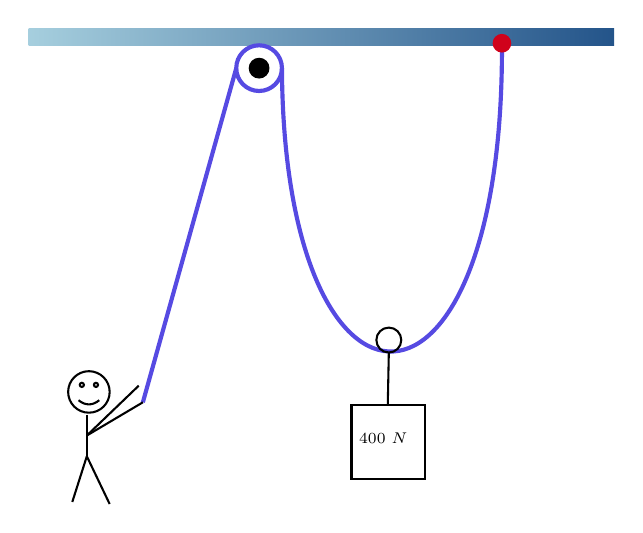
\begin{tikzpicture}[x=0.75pt,y=0.75pt,yscale=-1,xscale=1]
%uncomment if require: \path (0,300); %set diagram left start at 0, and has height of 300

%Shape: Rectangle [id:dp7610342163884872] 
\draw  [draw opacity=0][shading=_3v78oj4jj,_c80iqgthp] (1,11) -- (283,11) -- (283,19) -- (1,19) -- cycle ;
%Curve Lines [id:da7126596006092099] 
\draw [color={rgb, 255:red, 86; green, 74; blue, 226 }  ,draw opacity=1 ][line width=1.5]    (123,30) .. controls (124,214) and (230,214) .. (229,18) ;
%Shape: Circle [id:dp8605774160745977] 
\draw  [color={rgb, 255:red, 86; green, 74; blue, 226 }  ,draw opacity=1 ][line width=1.5]  (101,30) .. controls (101,23.92) and (105.92,19) .. (112,19) .. controls (118.08,19) and (123,23.92) .. (123,30) .. controls (123,36.08) and (118.08,41) .. (112,41) .. controls (105.92,41) and (101,36.08) .. (101,30) -- cycle ;
%Shape: Square [id:dp6540000147156467] 
\draw   (156.5,192.5) -- (192,192.5) -- (192,228) -- (156.5,228) -- cycle ;
%Shape: Circle [id:dp69331401971063] 
\draw   (168.5,161) .. controls (168.5,157.69) and (171.19,155) .. (174.5,155) .. controls (177.81,155) and (180.5,157.69) .. (180.5,161) .. controls (180.5,164.31) and (177.81,167) .. (174.5,167) .. controls (171.19,167) and (168.5,164.31) .. (168.5,161) -- cycle ;
%Straight Lines [id:da7057863663200589] 
\draw    (174.5,167) -- (174,192) ;
%Straight Lines [id:da5891185106727391] 
\draw [color={rgb, 255:red, 86; green, 74; blue, 226 }  ,draw opacity=1 ][line width=1.5]    (101,30) -- (56,191) ;
%Straight Lines [id:da8800202821656358] 
\draw    (29,197) -- (29,217) ;
%Straight Lines [id:da5861829155528433] 
\draw    (29,217) -- (40,240) ;
%Straight Lines [id:da893083642671363] 
\draw    (22,239) -- (29,217) ;
%Straight Lines [id:da2718809991809755] 
\draw    (29,207) -- (56,191) ;
%Straight Lines [id:da023130332312502278] 
\draw    (29,207) -- (54,183) ;
%Shape: Smiley Face [id:dp8427765858190384] 
\draw   (20,186) .. controls (20,180.48) and (24.48,176) .. (30,176) .. controls (35.52,176) and (40,180.48) .. (40,186) .. controls (40,191.52) and (35.52,196) .. (30,196) .. controls (24.48,196) and (20,191.52) .. (20,186) -- cycle ; \draw   (25.6,182.6) .. controls (25.6,182.05) and (26.05,181.6) .. (26.6,181.6) .. controls (27.15,181.6) and (27.6,182.05) .. (27.6,182.6) .. controls (27.6,183.15) and (27.15,183.6) .. (26.6,183.6) .. controls (26.05,183.6) and (25.6,183.15) .. (25.6,182.6) -- cycle ; \draw   (32.4,182.6) .. controls (32.4,182.05) and (32.85,181.6) .. (33.4,181.6) .. controls (33.95,181.6) and (34.4,182.05) .. (34.4,182.6) .. controls (34.4,183.15) and (33.95,183.6) .. (33.4,183.6) .. controls (32.85,183.6) and (32.4,183.15) .. (32.4,182.6) -- cycle ; \draw   (25,190) .. controls (28.33,192.67) and (31.67,192.67) .. (35,190) ;
%Shape: Circle [id:dp7648337593264566] 
\draw  [fill={rgb, 255:red, 0; green, 0; blue, 0 }  ,fill opacity=1 ] (107.5,30) .. controls (107.5,27.51) and (109.51,25.5) .. (112,25.5) .. controls (114.49,25.5) and (116.5,27.51) .. (116.5,30) .. controls (116.5,32.49) and (114.49,34.5) .. (112,34.5) .. controls (109.51,34.5) and (107.5,32.49) .. (107.5,30) -- cycle ;
%Shape: Circle [id:dp21825681009637454] 
\draw  [draw opacity=0][fill={rgb, 255:red, 208; green, 2; blue, 27 }  ,fill opacity=1 ] (224.5,18) .. controls (224.5,15.51) and (226.51,13.5) .. (229,13.5) .. controls (231.49,13.5) and (233.5,15.51) .. (233.5,18) .. controls (233.5,20.49) and (231.49,22.5) .. (229,22.5) .. controls (226.51,22.5) and (224.5,20.49) .. (224.5,18) -- cycle ;

% Text Node
\draw (159,204.4) node [anchor=north west][inner sep=0.75pt]  [font=\scriptsize,xscale=0.8,yscale=0.8]  {$400\ \text{N}$};


\end{tikzpicture}

    \caption{A $400\ \text N$ weight being distributed by one pulley.}
    \label{fig:pulley1}
\end{figure}
Here, a rope is carrying a $400\ \text N$ weight. Attached to the weight is a movable pulley, while the top pulley is fixed to the ceiling. Assuming an ideal (massless) rope and frictionless pulleys, the tension is the same everywhere in the rope. The movable pulley is supported by two rope segments, so the upward force on the load is $2T$. For the load to be held or lifted at constant speed,
$$2T = 400\ \text{N} \quad \Rightarrow \quad T = 200\ \text{N}$$

Assuming an ideal (massless) rope and frictionless pulleys, the tension is the same everywhere in the rope, so there is $200\ \text N$ throughout the rope. Since there are two ropes supporting the load, the Mechanical Advantage is $2$.

\begin{figure}[H]
    \centering


% Gradient Info
  
\tikzset {_z5lpa2xt8/.code = {\pgfsetadditionalshadetransform{ \pgftransformshift{\pgfpoint{0 bp } { 0 bp }  }  \pgftransformrotate{0 }  \pgftransformscale{2 }  }}}
\pgfdeclarehorizontalshading{_g32mfedn7}{150bp}{rgb(0bp)=(0.65,0.81,0.87);
rgb(37.5bp)=(0.65,0.81,0.87);
rgb(62.5bp)=(0.14,0.33,0.54);
rgb(100bp)=(0.14,0.33,0.54)}
\tikzset{every picture/.style={line width=0.75pt}} %set default line width to 0.75pt        

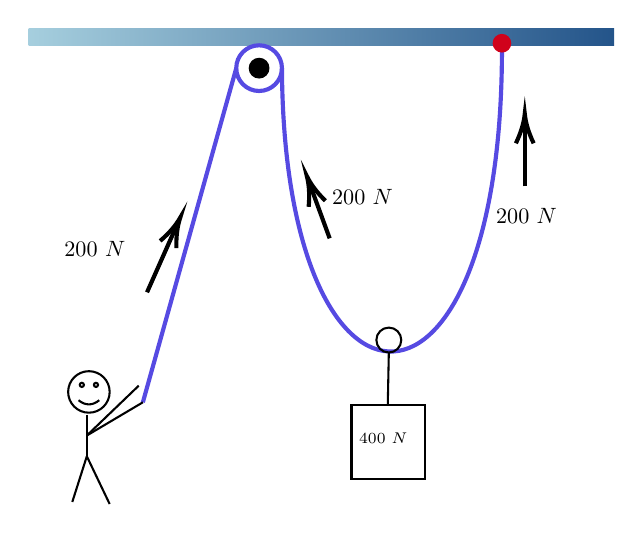
\begin{tikzpicture}[x=0.75pt,y=0.75pt,yscale=-1,xscale=1]
%uncomment if require: \path (0,300); %set diagram left start at 0, and has height of 300

%Shape: Rectangle [id:dp7610342163884872] 
\draw  [draw opacity=0][shading=_g32mfedn7,_z5lpa2xt8] (1,11) -- (283,11) -- (283,19) -- (1,19) -- cycle ;
%Curve Lines [id:da7126596006092099] 
\draw [color={rgb, 255:red, 86; green, 74; blue, 226 }  ,draw opacity=1 ][line width=1.5]    (123,30) .. controls (124,214) and (230,214) .. (229,18) ;
%Shape: Circle [id:dp8605774160745977] 
\draw  [color={rgb, 255:red, 86; green, 74; blue, 226 }  ,draw opacity=1 ][line width=1.5]  (101,30) .. controls (101,23.92) and (105.92,19) .. (112,19) .. controls (118.08,19) and (123,23.92) .. (123,30) .. controls (123,36.08) and (118.08,41) .. (112,41) .. controls (105.92,41) and (101,36.08) .. (101,30) -- cycle ;
%Shape: Square [id:dp6540000147156467] 
\draw   (156.5,192.5) -- (192,192.5) -- (192,228) -- (156.5,228) -- cycle ;
%Shape: Circle [id:dp69331401971063] 
\draw   (168.5,161) .. controls (168.5,157.69) and (171.19,155) .. (174.5,155) .. controls (177.81,155) and (180.5,157.69) .. (180.5,161) .. controls (180.5,164.31) and (177.81,167) .. (174.5,167) .. controls (171.19,167) and (168.5,164.31) .. (168.5,161) -- cycle ;
%Straight Lines [id:da7057863663200589] 
\draw    (174.5,167) -- (174,192) ;
%Straight Lines [id:da5891185106727391] 
\draw [color={rgb, 255:red, 86; green, 74; blue, 226 }  ,draw opacity=1 ][line width=1.5]    (101,30) -- (56,191) ;
%Straight Lines [id:da8800202821656358] 
\draw    (29,197) -- (29,217) ;
%Straight Lines [id:da5861829155528433] 
\draw    (29,217) -- (40,240) ;
%Straight Lines [id:da893083642671363] 
\draw    (22,239) -- (29,217) ;
%Straight Lines [id:da2718809991809755] 
\draw    (29,207) -- (56,191) ;
%Straight Lines [id:da023130332312502278] 
\draw    (29,207) -- (54,183) ;
%Shape: Smiley Face [id:dp8427765858190384] 
\draw   (20,186) .. controls (20,180.48) and (24.48,176) .. (30,176) .. controls (35.52,176) and (40,180.48) .. (40,186) .. controls (40,191.52) and (35.52,196) .. (30,196) .. controls (24.48,196) and (20,191.52) .. (20,186) -- cycle ; \draw   (25.6,182.6) .. controls (25.6,182.05) and (26.05,181.6) .. (26.6,181.6) .. controls (27.15,181.6) and (27.6,182.05) .. (27.6,182.6) .. controls (27.6,183.15) and (27.15,183.6) .. (26.6,183.6) .. controls (26.05,183.6) and (25.6,183.15) .. (25.6,182.6) -- cycle ; \draw   (32.4,182.6) .. controls (32.4,182.05) and (32.85,181.6) .. (33.4,181.6) .. controls (33.95,181.6) and (34.4,182.05) .. (34.4,182.6) .. controls (34.4,183.15) and (33.95,183.6) .. (33.4,183.6) .. controls (32.85,183.6) and (32.4,183.15) .. (32.4,182.6) -- cycle ; \draw   (25,190) .. controls (28.33,192.67) and (31.67,192.67) .. (35,190) ;
%Shape: Circle [id:dp7648337593264566] 
\draw  [fill={rgb, 255:red, 0; green, 0; blue, 0 }  ,fill opacity=1 ] (107.5,30) .. controls (107.5,27.51) and (109.51,25.5) .. (112,25.5) .. controls (114.49,25.5) and (116.5,27.51) .. (116.5,30) .. controls (116.5,32.49) and (114.49,34.5) .. (112,34.5) .. controls (109.51,34.5) and (107.5,32.49) .. (107.5,30) -- cycle ;
%Shape: Circle [id:dp21825681009637454] 
\draw  [draw opacity=0][fill={rgb, 255:red, 208; green, 2; blue, 27 }  ,fill opacity=1 ] (224.5,18) .. controls (224.5,15.51) and (226.51,13.5) .. (229,13.5) .. controls (231.49,13.5) and (233.5,15.51) .. (233.5,18) .. controls (233.5,20.49) and (231.49,22.5) .. (229,22.5) .. controls (226.51,22.5) and (224.5,20.49) .. (224.5,18) -- cycle ;
%Straight Lines [id:da009074770912673946] 
\draw [line width=1.5]    (58,138) -- (72.78,104.74) ;
\draw [shift={(74,102)}, rotate = 113.96] [color={rgb, 255:red, 0; green, 0; blue, 0 }  ][line width=1.5]    (14.21,-4.28) .. controls (9.04,-1.82) and (4.3,-0.39) .. (0,0) .. controls (4.3,0.39) and (9.04,1.82) .. (14.21,4.28)   ;
%Straight Lines [id:da35468354277363034] 
\draw [line width=1.5]    (146,112) -- (136.03,84.82) ;
\draw [shift={(135,82)}, rotate = 69.86] [color={rgb, 255:red, 0; green, 0; blue, 0 }  ][line width=1.5]    (14.21,-4.28) .. controls (9.04,-1.82) and (4.3,-0.39) .. (0,0) .. controls (4.3,0.39) and (9.04,1.82) .. (14.21,4.28)   ;
%Straight Lines [id:da7858167664551023] 
\draw [line width=1.5]    (240,87) -- (240,55) ;
\draw [shift={(240,52)}, rotate = 90] [color={rgb, 255:red, 0; green, 0; blue, 0 }  ][line width=1.5]    (14.21,-4.28) .. controls (9.04,-1.82) and (4.3,-0.39) .. (0,0) .. controls (4.3,0.39) and (9.04,1.82) .. (14.21,4.28)   ;

% Text Node
\draw (159,204.4) node [anchor=north west][inner sep=0.75pt]  [font=\scriptsize,xscale=0.8,yscale=0.8]  {$400\ \text{N}$};
% Text Node
\draw (225,96.4) node [anchor=north west][inner sep=0.75pt]  [xscale=0.8,yscale=0.8]  {$200\ \text{N}$};
% Text Node
\draw (146,87.4) node [anchor=north west][inner sep=0.75pt]  [xscale=0.8,yscale=0.8]  {$200\ \text{N}$};
% Text Node
\draw (17,112.4) node [anchor=north west][inner sep=0.75pt]  [xscale=0.8,yscale=0.8]  {$200\ \text{N}$};


\end{tikzpicture}
    \caption{The tension in the rope is $200 \ \text N$.}
    \label{fig:pulley2}
\end{figure}

However, this does come at a cost! The weight of the load is $400 \ \text N$ so the pulley system must provide a total upward force of $400 \ \text N$ on the load. However, both sections of rope (although technically the same rope) pull at $200 \ \text N$ for a total of $400 \ \text N$.

The work done, however, is still the same! When the person pulls the rope down by $2 \ \text m$, each supporting rope segment shortens by $1 \ \text m$, so the load rises by $1 \ \text m$. This is all ignoring friction and assuming constant speed.
Work done by the person:
$$W = F \times d = 200\,\text{N} \times 2\,\text{m} = 400\,\text{J}$$
Work gained by the load:
$$W = 400\,\text{N} \times 1\,\text{m} = 400\,\text{J}$$
This satisfies our work equation 
\begin{equation}
    \rm Work_{in} = Work_{out}
\end{equation}
Note that we can then rewrite our mechanical advantage as a proportion of distance:
\begin{equation}
    \text{MA} = \frac{d_{\text{effort}}}{d_{\text{load}}}
\end{equation}

\begin{Exercise}[title={Pulleys}, label={pulleysEX}]



% Gradient Info
  
\tikzset {_p5o42n8hj/.code = {\pgfsetadditionalshadetransform{ \pgftransformshift{\pgfpoint{0 bp } { 0 bp }  }  \pgftransformrotate{0 }  \pgftransformscale{2 }  }}}
\pgfdeclarehorizontalshading{_odt0ai6cz}{150bp}{rgb(0bp)=(0.65,0.81,0.87);
rgb(37.5bp)=(0.65,0.81,0.87);
rgb(62.5bp)=(0.14,0.33,0.54);
rgb(100bp)=(0.14,0.33,0.54)}
\tikzset{every picture/.style={line width=0.75pt}} %set default line width to 0.75pt        

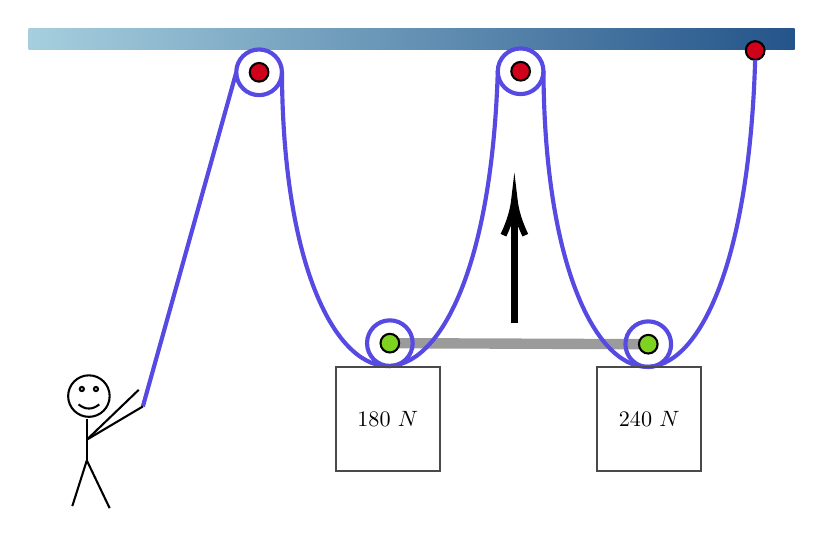
\begin{tikzpicture}[x=0.75pt,y=0.75pt,yscale=-1,xscale=1]
%uncomment if require: \path (0,300); %set diagram left start at 0, and has height of 300

%Straight Lines [id:da9180370752052216] 
\draw [color={rgb, 255:red, 155; green, 155; blue, 155 }  ,draw opacity=1 ][line width=3.75]    (299.5,161) -- (175,160.5) ;
%Shape: Rectangle [id:dp7610342163884872] 
\draw  [draw opacity=0][shading=_odt0ai6cz,_p5o42n8hj] (1,9) -- (370,9) -- (370,19) -- (1,19) -- cycle ;
%Curve Lines [id:da7126596006092099] 
\draw [color={rgb, 255:red, 86; green, 74; blue, 226 }  ,draw opacity=1 ][line width=1.5]    (123,30) .. controls (124,214) and (221,223.5) .. (227,29.5) ;
%Shape: Circle [id:dp8605774160745977] 
\draw  [color={rgb, 255:red, 86; green, 74; blue, 226 }  ,draw opacity=1 ][line width=1.5]  (101,30) .. controls (101,23.92) and (105.92,19) .. (112,19) .. controls (118.08,19) and (123,23.92) .. (123,30) .. controls (123,36.08) and (118.08,41) .. (112,41) .. controls (105.92,41) and (101,36.08) .. (101,30) -- cycle ;
%Straight Lines [id:da5891185106727391] 
\draw [color={rgb, 255:red, 86; green, 74; blue, 226 }  ,draw opacity=1 ][line width=1.5]    (101,30) -- (56,191) ;
%Straight Lines [id:da8800202821656358] 
\draw    (29,197) -- (29,217) ;
%Straight Lines [id:da5861829155528433] 
\draw    (29,217) -- (40,240) ;
%Straight Lines [id:da893083642671363] 
\draw    (22,239) -- (29,217) ;
%Straight Lines [id:da2718809991809755] 
\draw    (29,207) -- (56,191) ;
%Straight Lines [id:da023130332312502278] 
\draw    (29,207) -- (54,183) ;
%Shape: Smiley Face [id:dp8427765858190384] 
\draw   (20,186) .. controls (20,180.48) and (24.48,176) .. (30,176) .. controls (35.52,176) and (40,180.48) .. (40,186) .. controls (40,191.52) and (35.52,196) .. (30,196) .. controls (24.48,196) and (20,191.52) .. (20,186) -- cycle ; \draw   (25.6,182.6) .. controls (25.6,182.05) and (26.05,181.6) .. (26.6,181.6) .. controls (27.15,181.6) and (27.6,182.05) .. (27.6,182.6) .. controls (27.6,183.15) and (27.15,183.6) .. (26.6,183.6) .. controls (26.05,183.6) and (25.6,183.15) .. (25.6,182.6) -- cycle ; \draw   (32.4,182.6) .. controls (32.4,182.05) and (32.85,181.6) .. (33.4,181.6) .. controls (33.95,181.6) and (34.4,182.05) .. (34.4,182.6) .. controls (34.4,183.15) and (33.95,183.6) .. (33.4,183.6) .. controls (32.85,183.6) and (32.4,183.15) .. (32.4,182.6) -- cycle ; \draw   (25,190) .. controls (28.33,192.67) and (31.67,192.67) .. (35,190) ;
%Shape: Circle [id:dp7648337593264566] 
\draw  [fill={rgb, 255:red, 208; green, 2; blue, 27 }  ,fill opacity=1 ] (107.5,30) .. controls (107.5,27.51) and (109.51,25.5) .. (112,25.5) .. controls (114.49,25.5) and (116.5,27.51) .. (116.5,30) .. controls (116.5,32.49) and (114.49,34.5) .. (112,34.5) .. controls (109.51,34.5) and (107.5,32.49) .. (107.5,30) -- cycle ;
%Shape: Circle [id:dp11141198553472664] 
\draw  [color={rgb, 255:red, 86; green, 74; blue, 226 }  ,draw opacity=1 ][line width=1.5]  (164,160.5) .. controls (164,154.42) and (168.92,149.5) .. (175,149.5) .. controls (181.08,149.5) and (186,154.42) .. (186,160.5) .. controls (186,166.58) and (181.08,171.5) .. (175,171.5) .. controls (168.92,171.5) and (164,166.58) .. (164,160.5) -- cycle ;
%Shape: Circle [id:dp9019282353752629] 
\draw  [fill={rgb, 255:red, 126; green, 211; blue, 33 }  ,fill opacity=1 ] (170.5,160.5) .. controls (170.5,158.01) and (172.51,156) .. (175,156) .. controls (177.49,156) and (179.5,158.01) .. (179.5,160.5) .. controls (179.5,162.99) and (177.49,165) .. (175,165) .. controls (172.51,165) and (170.5,162.99) .. (170.5,160.5) -- cycle ;
%Shape: Circle [id:dp7460263183449106] 
\draw  [color={rgb, 255:red, 86; green, 74; blue, 226 }  ,draw opacity=1 ][line width=1.5]  (227,29.5) .. controls (227,23.42) and (231.92,18.5) .. (238,18.5) .. controls (244.08,18.5) and (249,23.42) .. (249,29.5) .. controls (249,35.58) and (244.08,40.5) .. (238,40.5) .. controls (231.92,40.5) and (227,35.58) .. (227,29.5) -- cycle ;
%Shape: Circle [id:dp19943929614254352] 
\draw  [fill={rgb, 255:red, 208; green, 2; blue, 27 }  ,fill opacity=1 ] (233.5,29.5) .. controls (233.5,27.01) and (235.51,25) .. (238,25) .. controls (240.49,25) and (242.5,27.01) .. (242.5,29.5) .. controls (242.5,31.99) and (240.49,34) .. (238,34) .. controls (235.51,34) and (233.5,31.99) .. (233.5,29.5) -- cycle ;
%Shape: Square [id:dp8917498304502549] 
\draw  [color={rgb, 255:red, 74; green, 74; blue, 74 }  ,draw opacity=1 ] (149,172) -- (199,172) -- (199,222) -- (149,222) -- cycle ;
%Shape: Circle [id:dp3181349974001967] 
\draw  [fill={rgb, 255:red, 208; green, 2; blue, 27 }  ,fill opacity=1 ] (346.5,19.5) .. controls (346.5,17.01) and (348.51,15) .. (351,15) .. controls (353.49,15) and (355.5,17.01) .. (355.5,19.5) .. controls (355.5,21.99) and (353.49,24) .. (351,24) .. controls (348.51,24) and (346.5,21.99) .. (346.5,19.5) -- cycle ;
%Shape: Circle [id:dp5973350274794632] 
\draw  [fill={rgb, 255:red, 126; green, 211; blue, 33 }  ,fill opacity=1 ] (295,161) .. controls (295,158.51) and (297.01,156.5) .. (299.5,156.5) .. controls (301.99,156.5) and (304,158.51) .. (304,161) .. controls (304,163.49) and (301.99,165.5) .. (299.5,165.5) .. controls (297.01,165.5) and (295,163.49) .. (295,161) -- cycle ;
%Curve Lines [id:da019076818267494633] 
\draw [color={rgb, 255:red, 86; green, 74; blue, 226 }  ,draw opacity=1 ][line width=1.5]    (249,29.5) .. controls (250,213.5) and (345,227) .. (351,24) ;
%Shape: Circle [id:dp07869876258534114] 
\draw  [color={rgb, 255:red, 86; green, 74; blue, 226 }  ,draw opacity=1 ][line width=1.5]  (288.5,161) .. controls (288.5,154.92) and (293.42,150) .. (299.5,150) .. controls (305.58,150) and (310.5,154.92) .. (310.5,161) .. controls (310.5,167.08) and (305.58,172) .. (299.5,172) .. controls (293.42,172) and (288.5,167.08) .. (288.5,161) -- cycle ;
%Shape: Square [id:dp25350547284915936] 
\draw  [color={rgb, 255:red, 74; green, 74; blue, 74 }  ,draw opacity=1 ] (275,172) -- (325,172) -- (325,222) -- (275,222) -- cycle ;
%Straight Lines [id:da7906341552791905] 
\draw [line width=2.25]    (235,151) -- (235,95) ;
\draw [shift={(235,91)}, rotate = 90] [color={rgb, 255:red, 0; green, 0; blue, 0 }  ][line width=2.25]    (17.49,-5.26) .. controls (11.12,-2.23) and (5.29,-0.48) .. (0,0) .. controls (5.29,0.48) and (11.12,2.23) .. (17.49,5.26)   ;

% Text Node
\draw (174,197) node  [xscale=0.8,yscale=0.8]  {$180\ \text{N}$};
% Text Node
\draw (300,197) node  [xscale=0.8,yscale=0.8]  {$240\ \text{N}$};


\end{tikzpicture}

A person is pulling 2 weights tensioned by 4 pulleys. There are 2 fixed pulleys (shown in red) and 2 movable pulleys (shown in green). The two movable pulleys are fixed such that they move together vertically. Calculate the input force that is needed to begin lifting the weights.

\end{Exercise}
\begin{Answer}[ref={pulleysEX}]
There are 4 segments supporting the net weight total of $420 \ \textrm{N}$. Each segment, then, splits the weight into $\dfrac{420 \ \rm N}{4} = 105 \ \rm N$. The input force required to move both weights is $105 \ \rm N$, which moves it $4 \ \rm m$. The output work matches as well: $420 \ \textrm{N}$ is moved $1 \ \rm m$.
\end{Answer}

\section{Wedges}
A wedge is a triangular shaped simple machine that converts forces from one direction to another. Often, it is from a vertical direction to a horizontal one. 

Similar to an inclined plane, wedges have steep angles to manipulate the properties of triangles. The force applied to the top portion of a wedge is transfered acting perpendicular to the sloped sides of the wedge.

\begin{figure}[H]
    \centering
\tikzset{every picture/.style={line width=0.75pt}} %set default line width to 0.75pt        

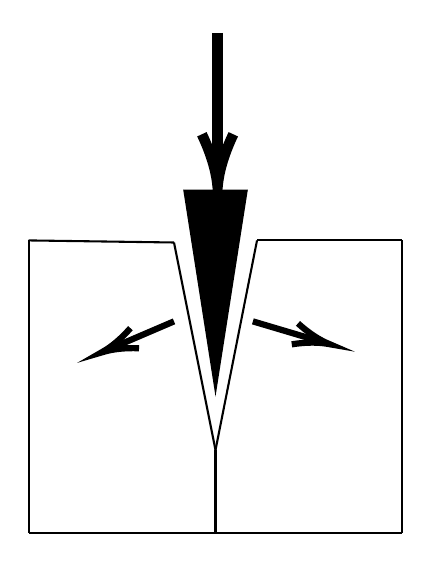
\begin{tikzpicture}[x=0.75pt,y=0.75pt,yscale=-1,xscale=1]
%uncomment if require: \path (0,300); %set diagram left start at 0, and has height of 300

%Shape: Triangle [id:dp6168998892540325] 
\draw  [fill={rgb, 255:red, 0; green, 0; blue, 0 }  ,fill opacity=1 ] (140,183) -- (155,87) -- (125,87) -- cycle ;
%Straight Lines [id:da8801497188706991] 
\draw    (50,111) -- (120,112) ;
%Straight Lines [id:da3144213400429735] 
\draw    (50,111) -- (50,252) ;
%Straight Lines [id:da8383979166880582] 
\draw    (120,112) -- (140,212) ;
%Straight Lines [id:da5091792831218536] 
\draw    (50,252) -- (140,252) ;
%Straight Lines [id:da9578263225604744] 
\draw    (140,212) -- (140,252) ;
%Straight Lines [id:da9587011857506123] 
\draw    (160,111) -- (230,111) ;
%Straight Lines [id:da8482644714627484] 
\draw    (230,111) -- (230,252) ;
%Straight Lines [id:da41416588926250886] 
\draw    (160,111) -- (140,212) ;
%Straight Lines [id:da17122520811836395] 
\draw    (140,252) -- (230,252) ;
%Straight Lines [id:da11907898239539394] 
\draw [line width=3.75]    (141,11) -- (141,79) ;
\draw [shift={(141,85)}, rotate = 270] [color={rgb, 255:red, 0; green, 0; blue, 0 }  ][line width=3.75]    (25.14,-7.57) .. controls (15.99,-3.21) and (7.61,-0.69) .. (0,0) .. controls (7.61,0.69) and (15.99,3.21) .. (25.14,7.57)   ;
%Straight Lines [id:da6900045763610622] 
\draw [line width=2.25]    (158,150) -- (191.17,159.86) ;
\draw [shift={(195,161)}, rotate = 196.56] [color={rgb, 255:red, 0; green, 0; blue, 0 }  ][line width=2.25]    (17.49,-5.26) .. controls (11.12,-2.23) and (5.29,-0.48) .. (0,0) .. controls (5.29,0.48) and (11.12,2.23) .. (17.49,5.26)   ;
%Straight Lines [id:da6375263453764765] 
\draw [line width=2.25]    (120,150) -- (88.68,163.42) ;
\draw [shift={(85,165)}, rotate = 336.8] [color={rgb, 255:red, 0; green, 0; blue, 0 }  ][line width=2.25]    (17.49,-5.26) .. controls (11.12,-2.23) and (5.29,-0.48) .. (0,0) .. controls (5.29,0.48) and (11.12,2.23) .. (17.49,5.26)   ;




\end{tikzpicture}

    \caption{A wedge splitting a block of wood, with the forces acting perpendicular.}
    \label{fig:wedges1}
\end{figure}

Similar to the inclined plane, the Mechanical Advantage is the proportion of the vertical rise or width, and the length of the sloped portion of the triangle.
\begin{equation}
   \rm MA = \frac{L}{V}
\end{equation}

The smaller the angle of a wedge, the greater the ratio of the length of its slope to its width, and the more mechanical advantage it will yield. This is a concept that comes directly from trigonometry.

\begin{Exercise}[title = {Wedges 1}, label = {wedgesEX}]
An axe is used to split wood. The length of the wedge is $12 \textrm{ cm}$ and the thickness is $3 \textrm{ cm}$. Calculate the mechanical advantage.
\end{Exercise}
\begin{Answer}[ref={wedgesEX}]

The mechanical advantage of the wedge is $\tfrac{12 \textrm{ cm}}{3 \textrm{ cm}} = 4$.

\end{Answer}

\begin{Exercise}[title={Wedges 2}, label={wedgesSA}]
Explain why a flathead-screwdriver tip is a poor option for cutting a steak compared to a knife.
\end{Exercise}
\begin{Answer}[ref={wedgesSA}]
A knife cuts better than a screwdriver tip because its edge is much thinner, giving it a greater mechanical advantage. This allows the applied force to be concentrated over a very small area, producing much higher pressure. As a result, less force is needed to cut the material. A screwdriver, on the other hand, has a very thick edge (in comparison), so its pressure and mechanical advantage are much less.
\end{Answer}
